\documentclass{article}

\usepackage{template/arxiv}
\usepackage{amsthm,amssymb,amsmath,amsfonts} % My additions
\usepackage[utf8]{inputenc} % allow utf-8 input
\usepackage[T1]{fontenc}    % use 8-bit T1 fonts
\usepackage[hidelinks]{hyperref} % hyperlinks
\usepackage{url}            % simple URL typesetting
\usepackage{booktabs}       % professional-quality tables
\usepackage{amsfonts}       % blackboard math symbols
\usepackage{nicefrac}       % compact symbols for 1/2, etc.
\usepackage{microtype}      % microtypography
\usepackage{cleveref}       % smart cross-referencing
\usepackage{lipsum}         % Can be removed after putting your text content

% My additions
\usepackage{graphicx}
\usepackage{natbib}
\usepackage{doi}
\graphicspath{ {./images/} } % MY
\newcommand{\vect}[1]{\mathbf{#1}} % vector notation % MY
\newcommand{\mat}[1]{\mathbf{#1}} % matrix notation % MY


\title{Analysis of IRS double reflection effect on users' rate and corresponding sum-rate}

% Here you can change the date presented in the paper title
%\date{September 9, 1985}
% Or remove it
\date{}


% Uncomment to use multiple affiliations variant of author block 
%\uniqueAffiliationtrue

% Multiple affiliations variant of author block
\usepackage{authblk}
\renewcommand\Authfont{\bfseries}
\setlength{\affilsep}{0em}
\author[1]{%
	\hspace{1mm}Alireza Tabatabaeian\thanks{alireza2541@aut.ac.ir}%
}
\author[1]{%
	\hspace{1mm}Danesh Abdollahi
}
\author[1]{%
	\hspace{1mm}Mohammad Sadegh Jafari
}
\author[1]{%
	\hspace{1mm}Mohammad Javad Emadi
}
\affil[1]{Department of Electrical Engineering, Amirkabir University of Technology (Tehran Polytechnic), Tehran, Iran}

% Uncomment to override  the `A preprint' in the header
\renewcommand{\headeright}{Arxiv Preprint}
\renewcommand{\undertitle}{Arxiv Preprint}
\renewcommand{\shorttitle}{\textit{arXiv} Preprint}

%%% Add PDF metadata to help others organize their library
%%% Once the PDF is generated, you can check the metadata with
%%% $ pdfinfo template.pdf
\hypersetup{
pdftitle={Analysis of IRS double reflection effect on users' rate and corresponding sum-rate},
pdfsubject={Intelligent Reflective Surface},
pdfauthor={Alireza Tabatabaeian},
pdfkeywords={IRS, Double Reflection, Sum-Rate, Coordinate Descent, Gradient Descent},
}

\begin{document}
\maketitle

\begin{abstract}
	This research explores the potential application of Intelligent Reflecting Surfaces (IRS) in the context of future communication networks, specifically focusing on 6G.
	The study aims to optimize the weighted-sum-rate objective function for a realistic scenario involving two users.
	In this scenario, the collaboration of two IRS units is considered, with a second-order reflection occurring between them.
	One of the users experiences an obstacle, highlighting the need for improved network performance.
	To enhance the communication network’s performance, a joint optimization approach is employed, optimizing both the passive beamforming coefficients of the IRS and the active beamforming coefficients of the antenna.
	This optimization is carried out using a coordinate descent algorithm consisting of a gradient descent inside it, which iteratively refines the beamforming coefficients to maximize the overall system performance. 
	The research also includes an evaluation of the Signal-to Interference-plus-Noise Ratio (SINR) improvement in the presence of the second-order reflection between the two IRS units.
	The optimization process comprises several key steps.
	Firstly, the Lagrangian dual transformation is applied to eliminate the logarithmic function, simplifying the optimization problem.
	This transformation facilitates a more efficient and tractable optimization process.
	Additionally, fractional programming techniques are employed to convert fractional terms into linear functions, further streamlining the optimization process.
	These optimization techniques enable the exploration of optimal beamforming strategies and pave the way for enhanced performance in future wireless communication systems.
\end{abstract}

% keywords can be removed
\keywords{IRS \and Double Reflection \and Sum-Rate \and Coordinate Descent \and Gradient Descent}

\section{Introduction}
The deployment of intelligent reflecting surfaces (IRS) in wireless communication systems has emerged as a promising technique to enhance the throughput and spectral efficiency. IRSs consist of a large number of reflective elements that can independently control the incident signals, enabling them to manipulate signal propagation. By strategically adjusting the phase shifts of these reflective elements, the IRS can shape the electromagnetic waves and achieve desired signal characteristics. This technology offers significant advantages, such as cost-effectiveness, low power consumption, and easy installation on various infrastructures. The integration of IRSs in 5G and 6G telecommunication wireless networks presents a new frontier in technology materials, revolutionizing the industry \cite{1}, \cite{2}. These surfaces can be attached to walls or windows, reflecting unused portions of electromagnetic waves to increase special rates in wireless communication, such as sum-rate or secrecy-rate.
\par In \cite{3}, it provides an overview of IRS fundamentals including signal models, hardware architectures, and practical constraints. It also discusses key design aspects of IRS-aided wireless systems such as Reflection optimization, Channel estimation and Deployment strategy.
The \cite{4} analyzes performance of IRS-aided communication between a single-antenna source and destination without a direct link, assisted by an IRS with M reflecting elements. Analytical expressions are derived for outage probability, symbol error rate, and achievable rate bounds. The analysis shows that the IRS can provide a diversity order equal to M. \cite{5} proposes a scalable optimization framework for configuring large intelligent reflecting surfaces (IRSs) in wireless communication systems. IRSs can shape wireless propagation environments by introducing configurable signal reflections.
To enable scalable optimization, the IRS unit cells are partitioned into tiles. The response of each tile is modeled using concepts from physics and electromagnetics. This avoids optimizing each unit cell individually. A two-stage optimization approach is proposed - an offline design stage creates a codebook of transmission modes for each tile, and an online optimization stage selects the best transmission mode for each tile to optimize system performance.
For an example multi-user downlink communication system, algorithms are proposed to minimize transmit power while ensuring quality of service for each user by jointly optimizing the IRS configuration and the transmitter beamforming.
\par \cite{6}, the paper studies a wireless communication system where a transmitter (Alice) sends confidential messages to two receivers ($Bob_r$ and $Bob_t$) in the presence of two eavesdroppers ($Eve_r$ and $Eve_t$). A simultaneously transmitting and reflecting reconfigurable intelligent surface (STAR-RIS) is deployed to enhance security by improving the legitimate channel and energy harvesting at the eavesdroppers. The STAR-RIS can dynamically adjust its transmission and reflection coefficients (TARCs) to control signal propagation. The achievable secrecy rate and harvested energy are derived as functions of the TARCs.
\par Also in \cite{7}, the paper studies using reconfigurable intelligent surfaces (RISs) to assist free-space optical (FSO) communications for providing broadband internet access to high-speed trains (HSTs).
An RIS can control and redirect incident light beams through tuning its transmission/reflection coefficients. This can extend coverage and improve link reliability compared to direct FSO links from base stations. Analytical models are derived for the end-to-end channel statistics of direct and RIS-assisted FSO links under weak and moderate-to-strong atmospheric turbulence conditions. Performance is analyzed in terms of average SNR and outage probability for two RIS coverage scenarios: fixed-oriented reflection (FOR) where each RIS cell has a fixed coverage zone, and dynamic-oriented reflection (DOR) where the RIS dynamically tracks and reflects to the HST position.
\par \cite{8}, \cite{9}, \cite{10}, \cite{11}  provide scenario for double reflection effect without considering the LoS effect.
\cite{8} Proposes a double-IRS aided wireless communication system with two distributed IRSs deployed near the base station (BS) and user.
Assumes a rank-1 line-of-sight (LoS) channel between the two IRSs and optimizes the passive beamforming design to achieve a power gain scaling with $K^4$, where K is the total number of IRS elements.
Simulation results validate the $K^4$ power scaling achieved by deploying two cooperative IRSs with optimized passive beamforming, which outperforms the $K^2$ scaling of a single IRS system. \cite{9} Studies channel estimation and passive beamforming design for a double-IRS aided single-user system. Proposes two channel estimation schemes: 1) estimates full channel matrix, 2) estimates two signature vectors for rank-1 LoS-dominant inter-IRS channel. Optimizes cooperative passive beamforming based on estimated channels to maximize achievable rate. Simulation results show significant rate enhancement of double-IRS system compared to single-IRS, especially with large number of elements.
\cite{10} Considers a double-IRS system where signals reach the user via cascaded BS-IRS1-IRS2-user link only.
Optimizes transmit and passive beamforming using particle swarm optimization to maximize received signal power.
Results show excellent signal-to-noise ratio can be achieved despite no direct BS-user link, demonstrating feasibility of communication via double IRS reflection.
\cite{11} Studies a double-IRS assisted multi-user MIMO system and proposes cooperative passive beamforming design. Analytically shows superior max SNR for single-user case and higher channel rank for multi-user case compared to single-IRS system. Proposes alternating optimization algorithm to maximize minimum SINR in multi-user case. Simulation results demonstrate significant rate gains of double-IRS system in various settings.
\par In summary, the four above papers study double-IRS assisted wireless communication systems under different system models and channel assumptions. The key focus is designing the cooperative passive beamforming over the two IRSs to achieve power scaling gains compared to single IRS systems. Both theoretical analysis and simulations demonstrate the performance gains of properly deployed double-IRS systems with optimized beamforming.

\par Notations: $x$ is scalar, $\vect{x}$ is vector, and $\mat{X}$ is matrix. Let $\mat{X}^T$, $\mat{X}^*$, and $\mat{X}^H$ denote the transpose, conjugate, and conjugate transpose of matrix $\mat{X}$, respectively. ${diag} (x_1, \ldots, x_n)$ represents a diagonal matrix with entries $x_1, \ldots, x_n$ on its main diagonal. $\mat{I}_M$ stands for $M \times M$ identity matrix. Operation ${Re}\{\mat{X}\}$ constructs a matrix by extracting the real parts of the entries of matrix $\mat{X}$, while operation $\angle(\mat{X})$ extracts the phases of elements of $\mat{X}$. The modulus of a complex number is denoted by $|\cdot|$, and $j = \sqrt{-1}$ is the imaginary unit. ${C}^{m \times n}$ represents the set of all $m \times n$ complex-valued matrices. Also the Hadamard product is denoted by $\odot$.
\par {\bf Organization}: The rest of this paper is organized as follows. 
In Section III, our proposed system model based on Double-Reflection-effect in IRS is introduced.
In Section IV, the sum-rate maximization problem subject to
power and unit modulus constraints is formulated.
In Section V, the proposed algorithm is described.
Numerical results are discussed in Section VI, and finally,
Section VII concludes the paper.

\section{Our Contribution}
At the moment, as you've seen, there are many papers and articles on the concept of intelligent reflecting surfaces. Not only a few of them considered the effect of double reflection or second-order reflection between IRS on the overall performance of the system, but also almost all of them neglect the effect of LoS in these scenarios applying an obstacle.
This neglecting was a motivation for us to propose a scenario to analyze the effect of double reflection in the presence of LoS signals. 
In this article, once and for all, we analyze the improvement achieved in the presence of double reflection to see that if it's rational to
neglect the double reflection effect or not.
\section{System Model}
- Without obstacle: In this scenario, both users have a direct line of sight to the antenna, and they also receive signals from both intelligent surfaces. Double reflection occurs between the intelligent surfaces. In this scenario, the weight of the users' reception rate is equal and set to a value of 1. Each user's receiver antenna has a single element, while the transmitting antenna has N elements. The intelligent surfaces, respectively, have $M_1$ and $M_2$ elements. In this scenario, each user receives signals from 5 different paths.

- With obstacle: In this scenario, only the second user has a direct line of sight to the antenna and receives signals from both intelligent surfaces. However, the first user does not have a direct line of sight to the transmitting antenna and only receives signals from first intelligent surface. Double reflection occurs between the intelligent surfaces. In this scenario, the weight of the users' reception rate is equal and set to a value of 1, but if needed, the weight of the first user can be increased due to receiving fewer signals. Each user's receiver antenna has a single element, while the transmitting antenna has N elements. The intelligent surfaces, respectively, have $M_1$ and $M_2$ elements. In this scenario, the first user receives signals from 2 paths, and the second user receives signals from 5 different paths, as depicted in the following diagram:

\begin{figure}[!h]
	\centering
	\begin{minipage}{.5\textwidth}
		\flushleft		
		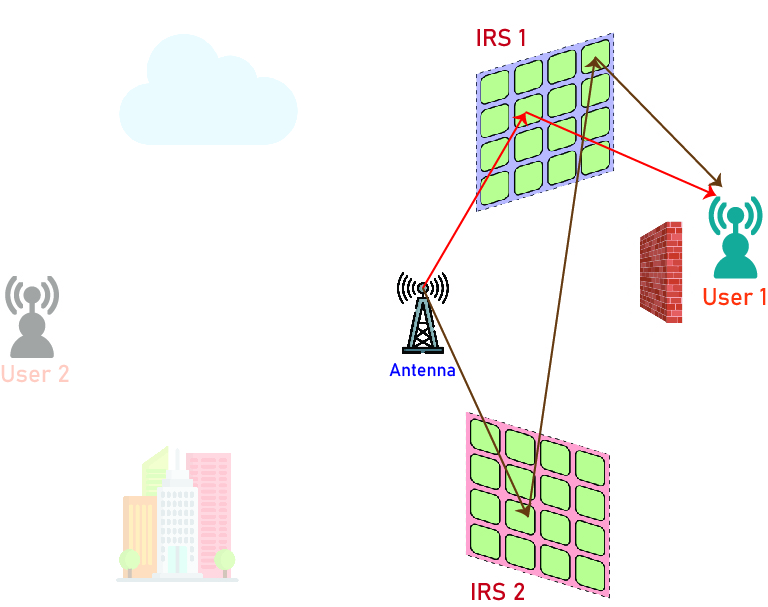
\includegraphics[width=0.9\linewidth]{with_obstacle__user1}
		\caption{First User's Links}
	\end{minipage}%
	\vline
	\begin{minipage}{.5\textwidth}
		\flushright
		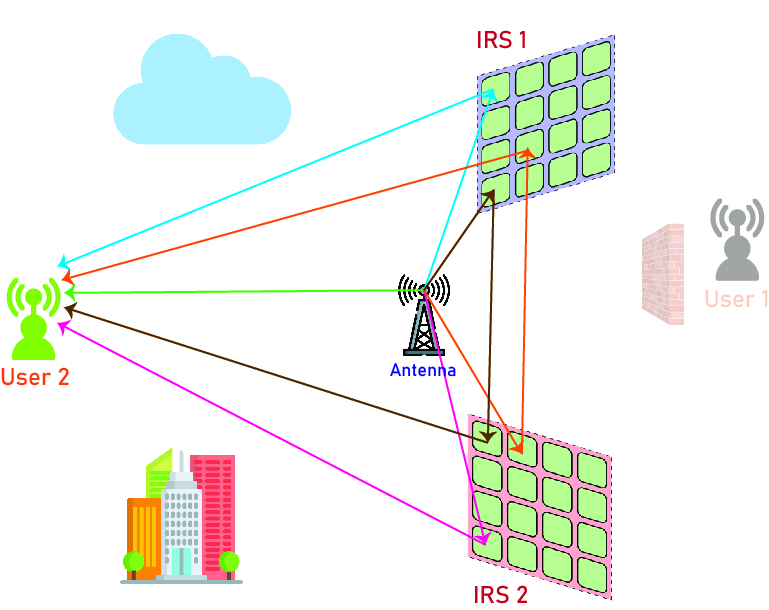
\includegraphics[width=0.9\linewidth]{with_obstacle__user2}
		\caption{Second User's Links}
	\end{minipage}
\end{figure}

\subsection{Received Signal at \boldmath{$k$}-th user}
Denote the transmit data symbol to user $k$ by $s_k$. It is assumed that $s_k$ ($k = 1, \ldots, K$) are independent random variables with zero mean and unit variance. Then, the transmitted signal at the BS can be expressed as
\begin{equation}
	x = \sum_{k=1}^{K} w_k s_k, \label{eq:transmitted_signal}
\end{equation}
where $w_k \in \mathbb{C}^{N_t \times 1}$ is the corresponding transmit beamforming vector.

The received signal at user $k$ without considering the obstacles can be expressed as:

\begin{align*}
	y_k = &\underbrace{h_{d,k}^H x}_
	{\substack{\text{Direct link}}}
	\quad + \quad \\
	&\underbrace{h_{r_1,k}^H \Phi_1 G_1 x}_
	{\substack{\text{IRS1 link}}}
	\quad + \quad
	\underbrace{h_{r_2,k}^H \Phi_2 G_2 x}_
	{\substack{\text{IRS2 link}}}
	\quad + \quad \\ 
	&\underbrace{h_{r_1,k}^H \Phi_1 D \Phi_2 G_2 x}_
	{\substack{\text{Double reflection link}}}
	\quad + \quad
	\underbrace{h_{r_2,k}^H \Phi_2 D^H \Phi_1 G_1 x}_
	{\substack{\text{Double reflection link}}} \quad + \quad
	\underbrace{u_k}_
	{\substack{\text{AWGN}}}
\end{align*}

where $u_k \sim \mathcal{CN}(0, \sigma_0^2)$ denotes the additive white Gaussian noise (AWGN) at the $k$-th user receiver.

\subsection{SINR and Rate at \boldmath{$k$}-th user}
The $k$-th user treats all the signals from other users (i.e.,
$s_1$, ... , $s_{k-1}$, $s_{k+1}$, ... , $s_K$) as interference. Hence, the decoding SINR of $s_k$ at user $k$ is

\[
\gamma_k = \frac{{\left|\left(h_{d,k}^H + h_{r_1,k}^H \Phi_1 G_1 + h_{r_2,k}^H \Phi_2 G_2 + h_{r_1,k}^H \Phi_1 D \Phi_2 G_2 + h_{r_2,k}^H \Phi_2 D^H \Phi_1 G_1 \right)w_k\right|^2}}{{\sum_{i=1,i\neq k}^{K} \left|\left(h_{d,k}^H + h_{r_1,k}^H \Phi_1 G_1 + h_{r_2,k}^H \Phi_2 G_2 + h_{r_1,k}^H \Phi_1 D \Phi_2 G_2 + h_{r_2,k}^H \Phi_2 D^H \Phi_1 G_1 \right)w_i\right|^2 + \sigma^2_0}}
\]

and the sum-rate of users are:
\[Rate = \sum_{k=1}^{K} \omega_k \log_2(1 + \gamma_k)\]

\section{Problem Formulation}
In this project, the objective is to maximize the total user reception rate, referred to as the WSR (Weighted Sum Rate). To achieve this, it is necessary to simultaneously and jointly optimize the antenna coefficients and the phase coefficients of the intelligent surfaces because these two categories of variables influence each other and cannot be optimized separately. Additionally, any solution proposed for the antenna coefficients must satisfy the power constraint condition.

\subsection{Objective Function and constraints}
The problem can be formulated as follows:
\begin{align*}
	(P1) \quad \max_{\mathbf{W}, \boldsymbol{\Phi_1}, \boldsymbol{\Phi_2}} \quad & f_1(\mathbf{W}, \boldsymbol{\Phi_1}, \boldsymbol{\Phi_2}) = \sum_{k=1}^{K} \omega_k \log_2(1 + \gamma_k) \\
	\text{s.t.} \quad & \theta_{m_k} \in \mathcal{F}, \quad \forall m_k = 1, \ldots, M_k, \\
	& \sum_{k=1}^{K} \| \mathbf{w}_k \|_2^2 \leq P_T,
\end{align*}

The transmit power constraint of BS is:
\[
\sum_{k=1}^{K} ||w_k||^2 \leq P_T
\]

and the $\mathcal{F}$ is the unit-module also known as the unit ball where the IRS coefficients belong to.

\section{Proposed Algorithm}
In this section, we will define the "Alternating Optimization" algorithm, also known as the "Coordinate Descent" algorithm, and explain how it is used. The Alternating Optimization algorithm is a technique commonly employed in optimization problems where multiple variables are involved, and optimizing them jointly is challenging. Instead of optimizing all variables simultaneously, this approach alternates between optimizing one variable while keeping the others fixed.

Step 1: Antenna Coefficients Optimization

Initialize the phase coefficients of the intelligent surfaces.
Optimize the antenna coefficients while keeping the phase coefficients fixed. This step focuses on finding the best values for the antenna coefficients while assuming that the phase coefficients are constant.
Once the antenna coefficients are optimized, they are treated as fixed values for the next step.

Step 2: Phase Coefficients Optimization

Initialize the phase coefficients of the intelligent surfaces (which were optimized in step 1). Optimize the phase coefficients while keeping the antenna coefficients fixed. This step focuses on finding the best values for the phase coefficients while assuming that the antenna coefficients are constant.

\subsection{Lagrangian Dual Transformation}
As mentioned in \cite{13}, \cite{14}, one of the challenges encountered in this optimization problem, as well as in all problems related to optimizing maximum achievable rates, is the presence of logarithmic functions. If there was only a single logarithmic function, it could have been eliminated because the logarithm function is strictly monotonically increasing. Therefore, we could have optimized the function inside the logarithm directly. However, in this case, we are dealing with the summation of multiple logarithmic functions.


Now that we understand the challenge, let's move on to one of the most well-known solutions. One of the transformations that can be used to eliminate logarithmic functions in such problems is the logarithmic dual transformation. This transformation was introduced by two prominent members of the electrical engineering community in 2018, in the second part of a paper aimed at solving telecommunications problems.

The technique involves introducing optional parameters called "alpha" to the problem. By doing so, it displaces the function in front of the logarithm, effectively simplifying the optimization problem by eliminating the logarithm. We will continue to use this widely used technique in the following way:

Our 4-2 problem can be transformed to the following problem:
\[
f_{1a}(\mathbf{W}, \boldsymbol{\Theta}, \boldsymbol{\alpha}) = \sum_{k=1}^{K} \omega_k \log_2(1 + \alpha_k) - \sum_{k=1}^{K} \omega_k \alpha_k + \sum_{k=1}^{K} \frac{\omega_k (1 + \alpha_k) \gamma_k}{1 + \gamma_k}
\]

As it's obvious, we've added auxiliary variable $\alpha_k$ such that $k = 1 ... K$ where K is the number of users.

Also, $\gamma_k$ represents the signal-to-noise ratio. Now, you might wonder how adding a new set of parameters can simplify the problem. The answer to this question becomes clear when we start optimizing these two sets of parameters using the coordinate descent algorithm:

The first set consists of antenna and intelligent surface parameters.
The second set includes the newly added optional parameters.
To achieve this, we first assume the first set of parameters to be fixed and take derivatives with respect to the second set of parameters. Importantly, this differentiation can be easily performed, and by setting it to zero, we find the optimal value for alpha as follows:
\[\alpha_k^\circ = \gamma_k\]

Now, with alpha assumed to be constant, the problem is 
transformed as follows:
\[
\quad \max \mathbf{W}, \boldsymbol{\Theta} \quad \sum_{k=1}^{K} \frac{\alpha_k^\sim \gamma_k}{1 + \gamma_k}
\]
such that $\alpha_k^\sim = \omega_k(1 + \alpha_k)$

Now, we have a sum of several fractional expressions. In the following section, we will use the technique of fractional programming to solve this problem.

\subsection{Multiple-ratio Fractional Programming}
Now, as mentioned in \cite{12}, we are dealing with several fractions that are not easily differentiable, and solving the resulting equation is not straightforward. Therefore, it's necessary to use another transformation called "fractional programming" to convert this problem into a linear form, in such a way that the resulting problem is equivalent to the original problem, meaning they have the same optimal solutions.

This transformation, as introduced in the first part of the paper mentioned in the previous section, is similar to the transformation discussed earlier and other transformations. It involves adding an optional set of parameters called "beta" to the problem, which, of course, simplifies the optimization problem.
Next, we will discuss how to apply this technique to the problem.

First, for the sake of clarity in the writing, we define a new parameter related to the channels:
\[\mathbf{h}_k = \mathbf{h}_{d,k} + \mathbf{GH}\boldsymbol{\Theta}\mathbf{h}_{r,k}\]

So, the signal-to-noise-plus-interference ratio (SINR) changes as follows:

\[
\gamma_k = \frac{{\lVert \mathbf{h}_k \mathbf{w}_k \rVert^2}}{{\sum_{i=1,i\neq k}^{K} \lVert \mathbf{h}_k \mathbf{w}_i \rVert^2 + \sigma_0^2}}
\]

Now, by using the fractional programming transformation and introducing the parameter beta, the optimization problem changes as follows and is written in linear form:
\[
f2a(\mathbf{W}, \boldsymbol{\beta}) = \sum_{k=1}^{K} 2 \sqrt{\alpha_k^\sim} \Re \left\{ \beta_k^* \mathbf{h}_k^H \mathbf{w}_k \right\} - \sum_{k=1}^{K} \lvert \beta_k \rvert^2 \sum_{i=1}^{K} \lVert \mathbf{h}_k \mathbf{w}_i \rVert^2 + \sigma_0^2.
\]

In such a way that the domain of beta is equal to complex numbers.

Now, once again, by employing the coordinate descent algorithm we can optimize the parameters, including beta, and other parameters within a loop.
To do this, we first take the derivative with respect to beta and find its optimal value. This can be easily accomplished.
The optimal value of beta is provided below:
\[
\beta_k^* = \sqrt{\alpha_k^\sim} \frac{{\mathbf{h}_k^H \mathbf{w}_k}}{{\sum_{i=1}^{K} \lVert \mathbf{h}_k \mathbf{w}_i \rVert^2 + \sigma_0^2}}.
\]

\subsection{Active Beamforming Optimization}
Now it's time to optimize the first set of primary parameters in the problem, namely the antenna coefficients. Similar to other parameters, to find their optimal values, we take the derivative with respect to W and set it equal to zero. The result is shown in the equation below:

\[\mathbf{w}_k^* = \sqrt{\alpha_k^\sim} \beta_k \left( \lambda_0 \mathbf{I}_M + \sum_{i=1}^{K} \lvert \beta_i \rvert^2 \mathbf{h}_i \mathbf{h}_i^H \right)^{-1} \mathbf{h}_k,
\]

However, it's worth mentioning that since we need to satisfy a power constraint on this set of parameters, we must add an auxiliary parameter named lambda to the problem. By adjusting lambda, we can enforce the power constraint. The optimal value of lambda is obtained by solving the following equation:

\[
\lambda_0^* = \min \left( \lambda_0 \geq 0 : \sum_{k=1}^{K} \lVert \mathbf{w}_k \rVert^2 \leq PT \right).
\]

Solving this inequality can be achieved using a binary search (also known as bisection search) algorithm.

\subsection{Passive Beamforming Optimization}
Now we move on to optimizing the second set of primary parameters in the problem. Again, to convert fractions into linear expressions, we need to utilize fractional programming, as shown below (this time with the parameter epsilon):

\[
f_{3 a}(\boldsymbol{\theta}, \boldsymbol{\varepsilon})=  \sum_{k=1}^{K} 2 \sqrt{\tilde{\alpha}_{k}} \operatorname{Re}\left\{\varepsilon_{k}^{*} \boldsymbol{\theta}^{\mathrm{H}} \mathbf{a}_{k, k}+\varepsilon_{k}^{*} b_{k, k}\right\} \\
-\sum_{k=1}^{K}\left|\varepsilon_{k}\right|^{2}\left(\sum_{i=1}^{K}\left|b_{i, k}+\boldsymbol{\theta}^{\mathrm{H}} \mathbf{a}_{i, k}\right|^{2}+\sigma_{0}^{2}\right)
\]

Just like in the previous section where we found the optimal value of beta, now we proceed to calculate the optimal value of epsilon:

\[
\varepsilon_{k}^{\circ}=\frac{\sqrt{\tilde{\alpha}_{k}}\left(b_{k, k}+\boldsymbol{\theta}^{\mathrm{H}} \mathbf{a}_{k, k}\right)}{\sum_{i=1}^{K}\left|b_{i, k}+\boldsymbol{\theta}^{\mathrm{H}} \mathbf{a}_{i, k}\right|^{2}+\sigma_{0}^{2}} .
\]

To calculate the optimal value of theta, we can take derivatives again, but this method can be slow. It's better to use the gradient descent method for a vector. First, let's provide a few simple definitions:

\[
\left|b_{i, k}+\boldsymbol{\theta}^{\mathrm{H}} \mathbf{a}_{i, k}\right|^{2}  =\left(b_{i, k}+\boldsymbol{\theta}^{\mathrm{H}} \mathbf{a}_{i, k}\right)\left(b_{i, k}^{*}+\mathbf{a}_{i, k}^{\mathrm{H}} \boldsymbol{\theta}\right) \\
=\boldsymbol{\theta}^{\mathrm{H}} \mathbf{a}_{i, k} \mathbf{a}_{i, k}^{\mathrm{H}} \boldsymbol{\theta}+2 \operatorname{Re}\left\{b_{i, k}^{*} \boldsymbol{\theta}^{\mathrm{H}} \mathbf{a}_{i, k}\right\}+\left|b_{i, k}\right|^{2}
\]

\[	f_{4}(\boldsymbol{\theta})  =f_{3 a}\left(\boldsymbol{\theta}, \boldsymbol{\varepsilon}^{\circ}\right) \\
=-\boldsymbol{\theta}^{\mathrm{H}} \boldsymbol{R} \boldsymbol{\theta}+2 \operatorname{Re}\left\{\boldsymbol{\theta}^{\mathrm{H}} \boldsymbol{e}\right\}+C,
\]

\[	\boldsymbol{R}  =\sum_{k=1}^{K}\left|\varepsilon_{k}\right|^{2} \sum_{i=1}^{K} \mathbf{a}_{i, k} \mathbf{a}_{i, k}^{\mathrm{H}},
\]

\[
\boldsymbol{e}  =\sum_{k=1}^{K}\left(\sqrt{\tilde{\alpha}_{k}} \varepsilon_{k}^{*} \mathbf{a}_{k, k}-\left|\varepsilon_{k}\right|^{2} \sum_{i=1}^{K} b_{i, k}^{*} \mathbf{a}_{i, k}\right),
\]

\[
C  =\sum_{k=1}^{K}\left(2 \sqrt{\tilde{\alpha}_{k}} \operatorname{Re}\left\{\varepsilon_{k}^{*} b_{k, k}\right\}-\left|\varepsilon_{k}\right|^{2}\left(\sigma_{0}^{2}+\sum_{i=1}^{K}\left|b_{i, k}\right|^{2}\right)\right)
\]

First, as mentioned in \cite{15}, using gradient descent and mapping the solution onto the unit circle, we can calculate the gradient value through the following equation:

\[
\nabla_{\Theta} f_{4}=2 \operatorname{Re}\left\{(\mathbf{R \theta}-\mathbf{e})^{*} \odot(-j \mathbf{\theta})\right\},
\]

Now, using the concept of iterative gradient descent, we can obtain the new value of the phase coefficients for intelligent surface number 1 as a combination of the previous value along with a coefficient times the changes (gradients) through the following equation:

\[
\boldsymbol{\Theta}^{(t+1)}=\boldsymbol{\Theta}^{(t)}-\gamma^{(t)} \nabla_{\boldsymbol{\Theta}} f\left(\mathbf{X}^{(t)}\right),
\]

Calculating the coefficients for intelligent surface number 2 can also be done using a similar method.

For optimizing the phase coefficients, there are three main regions where the final solution can be mapped:

Region 1: This is the inside region of the unit circle, where most algorithms typically start converging. However, solutions in this region may not be the global optimum because they often come with a reduction in power (the magnitude of the vector inside the unit circle is less than 1).

Region 2: This region corresponds to points on the unit circle. The likelihood of finding the global optimum in this region is higher. Solutions obtained inside the unit circle can be mapped to this region by normalizing their vector magnitude to 1.

Region 3: This region is the quantized region on the unit circle. It is a subset of the previous region and contains a limited set of points. For example, a 9-bit quantization can be applied, resulting in approximately one degree of error.

The problem is typically solved in Region 2, which can easily be mapped to the nearest point in Region 3 during implementation.

\section{Numerical Results}
In this section, we simulate the scenario in two cases, one without obstacles and the other with obstacles. To do this, we set the necessary parameters in the simulation as follows, and we run the simulation 10 times for each $M_1$ simulations, with each $M_1$ being a multiple of 10, and then we analyze the results to generate the following charts. The given parameters in the simulation are as follows:

- Number of antenna elements: N = 20

- Number of elements in the second intelligent surface: $M_2$ = 20

- Weight of user rate: 1

- Total power of two users: 10 mW

- Gaussian Noise standard deviation: 0.0001

- Direct path power loss coefficient: 2.5

- Power path loss coefficient between antenna and intelligent surfaces or intelligent surfaces and users: 2

- Power path loss coefficient between intelligent surfaces: 1.8

- Distance from user 1 to antenna: 50 meters

- Distance from user 2 to antenna: 60 meters

- Distance from intelligent surface 1 to antenna: 20 meters

- Distance from intelligent surface 2 to antenna: 30 meters

- Distance from user 1 to intelligent surface 1: 150 meters

- Distance from user 1 to intelligent surface 2: 230 meters

- Distance from user 2 to intelligent surface 1: 140 meters

- Distance from user 2 to intelligent surface 2: 220 meters

- Distance between intelligent surfaces: 40 meters

- Gradient Descent Step Size: 0.1

\subsection{Without Obstacle}
According to the conditions mentioned and in the absence of obstacles, simulations were conducted, and the following plots represent the user rates for User 1, User 2, and the total rate for both users:

\begin{figure}[!h]
	\centering
	\begin{minipage}{.5\textwidth}
		\flushleft
		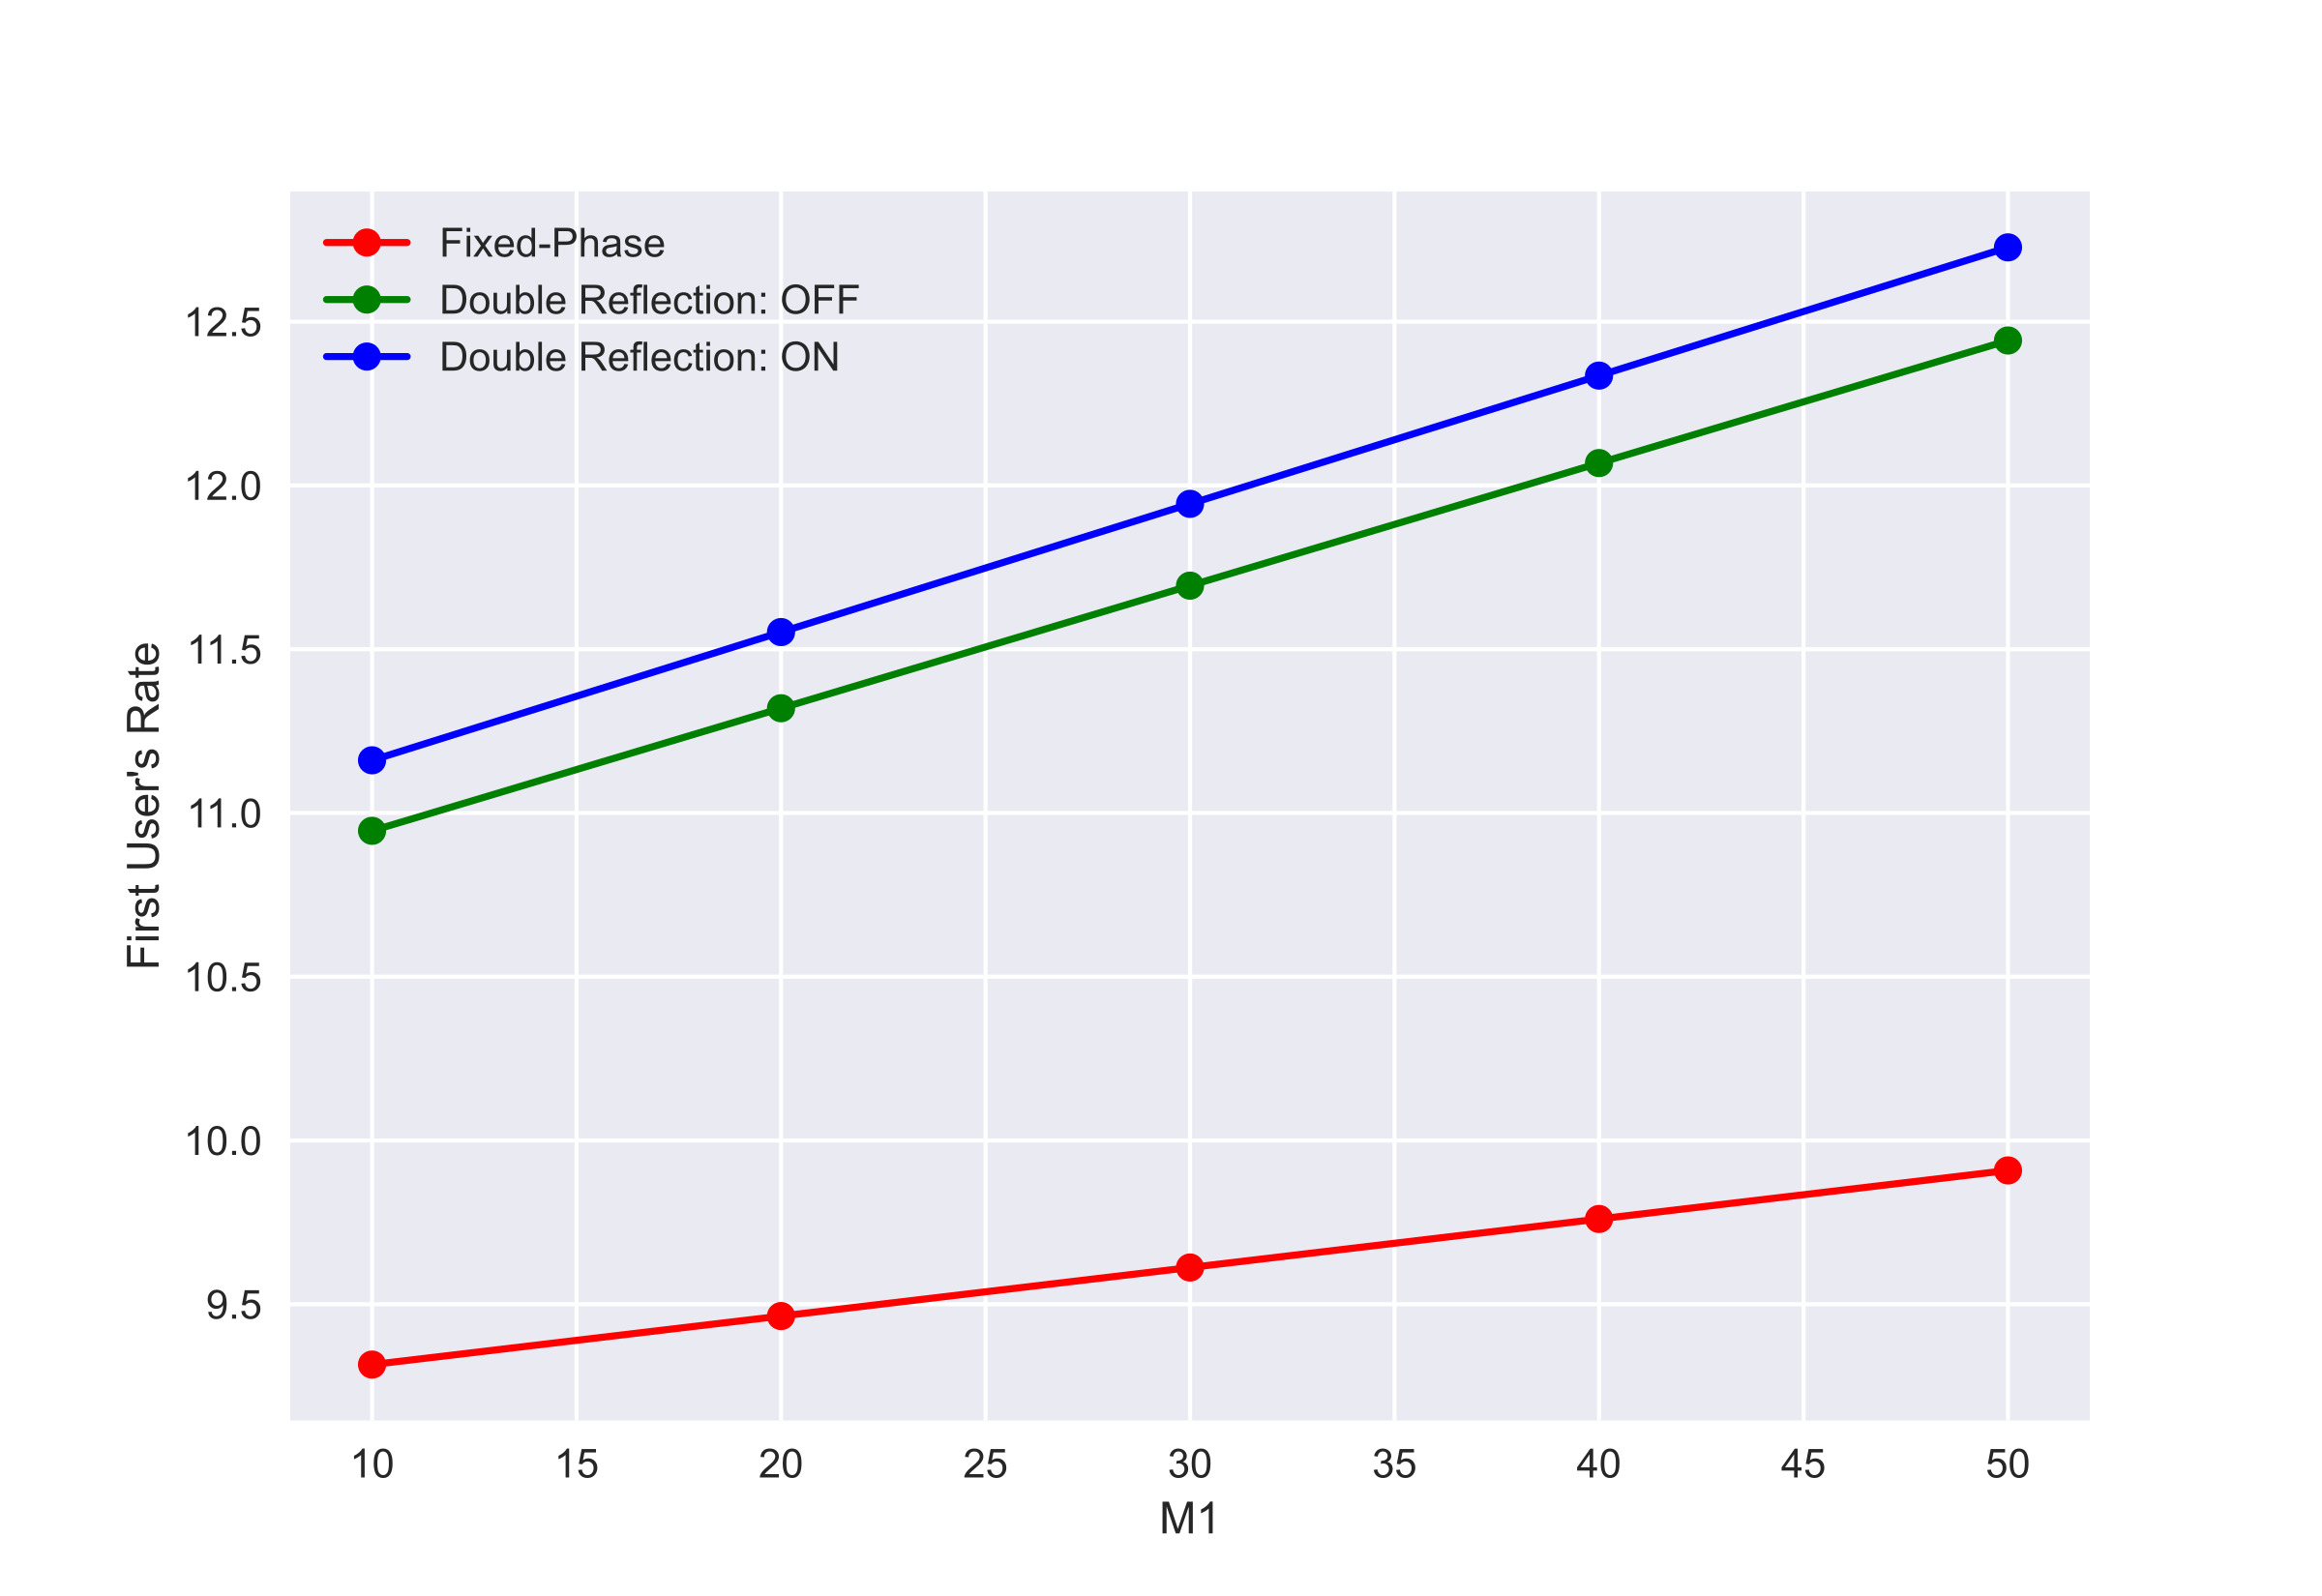
\includegraphics[width=0.95\linewidth]{No Blockage First User's Rate}
		\caption{First User's Rate}
	\end{minipage}%
	\vline
	\begin{minipage}{.5\textwidth}
		\flushright			
		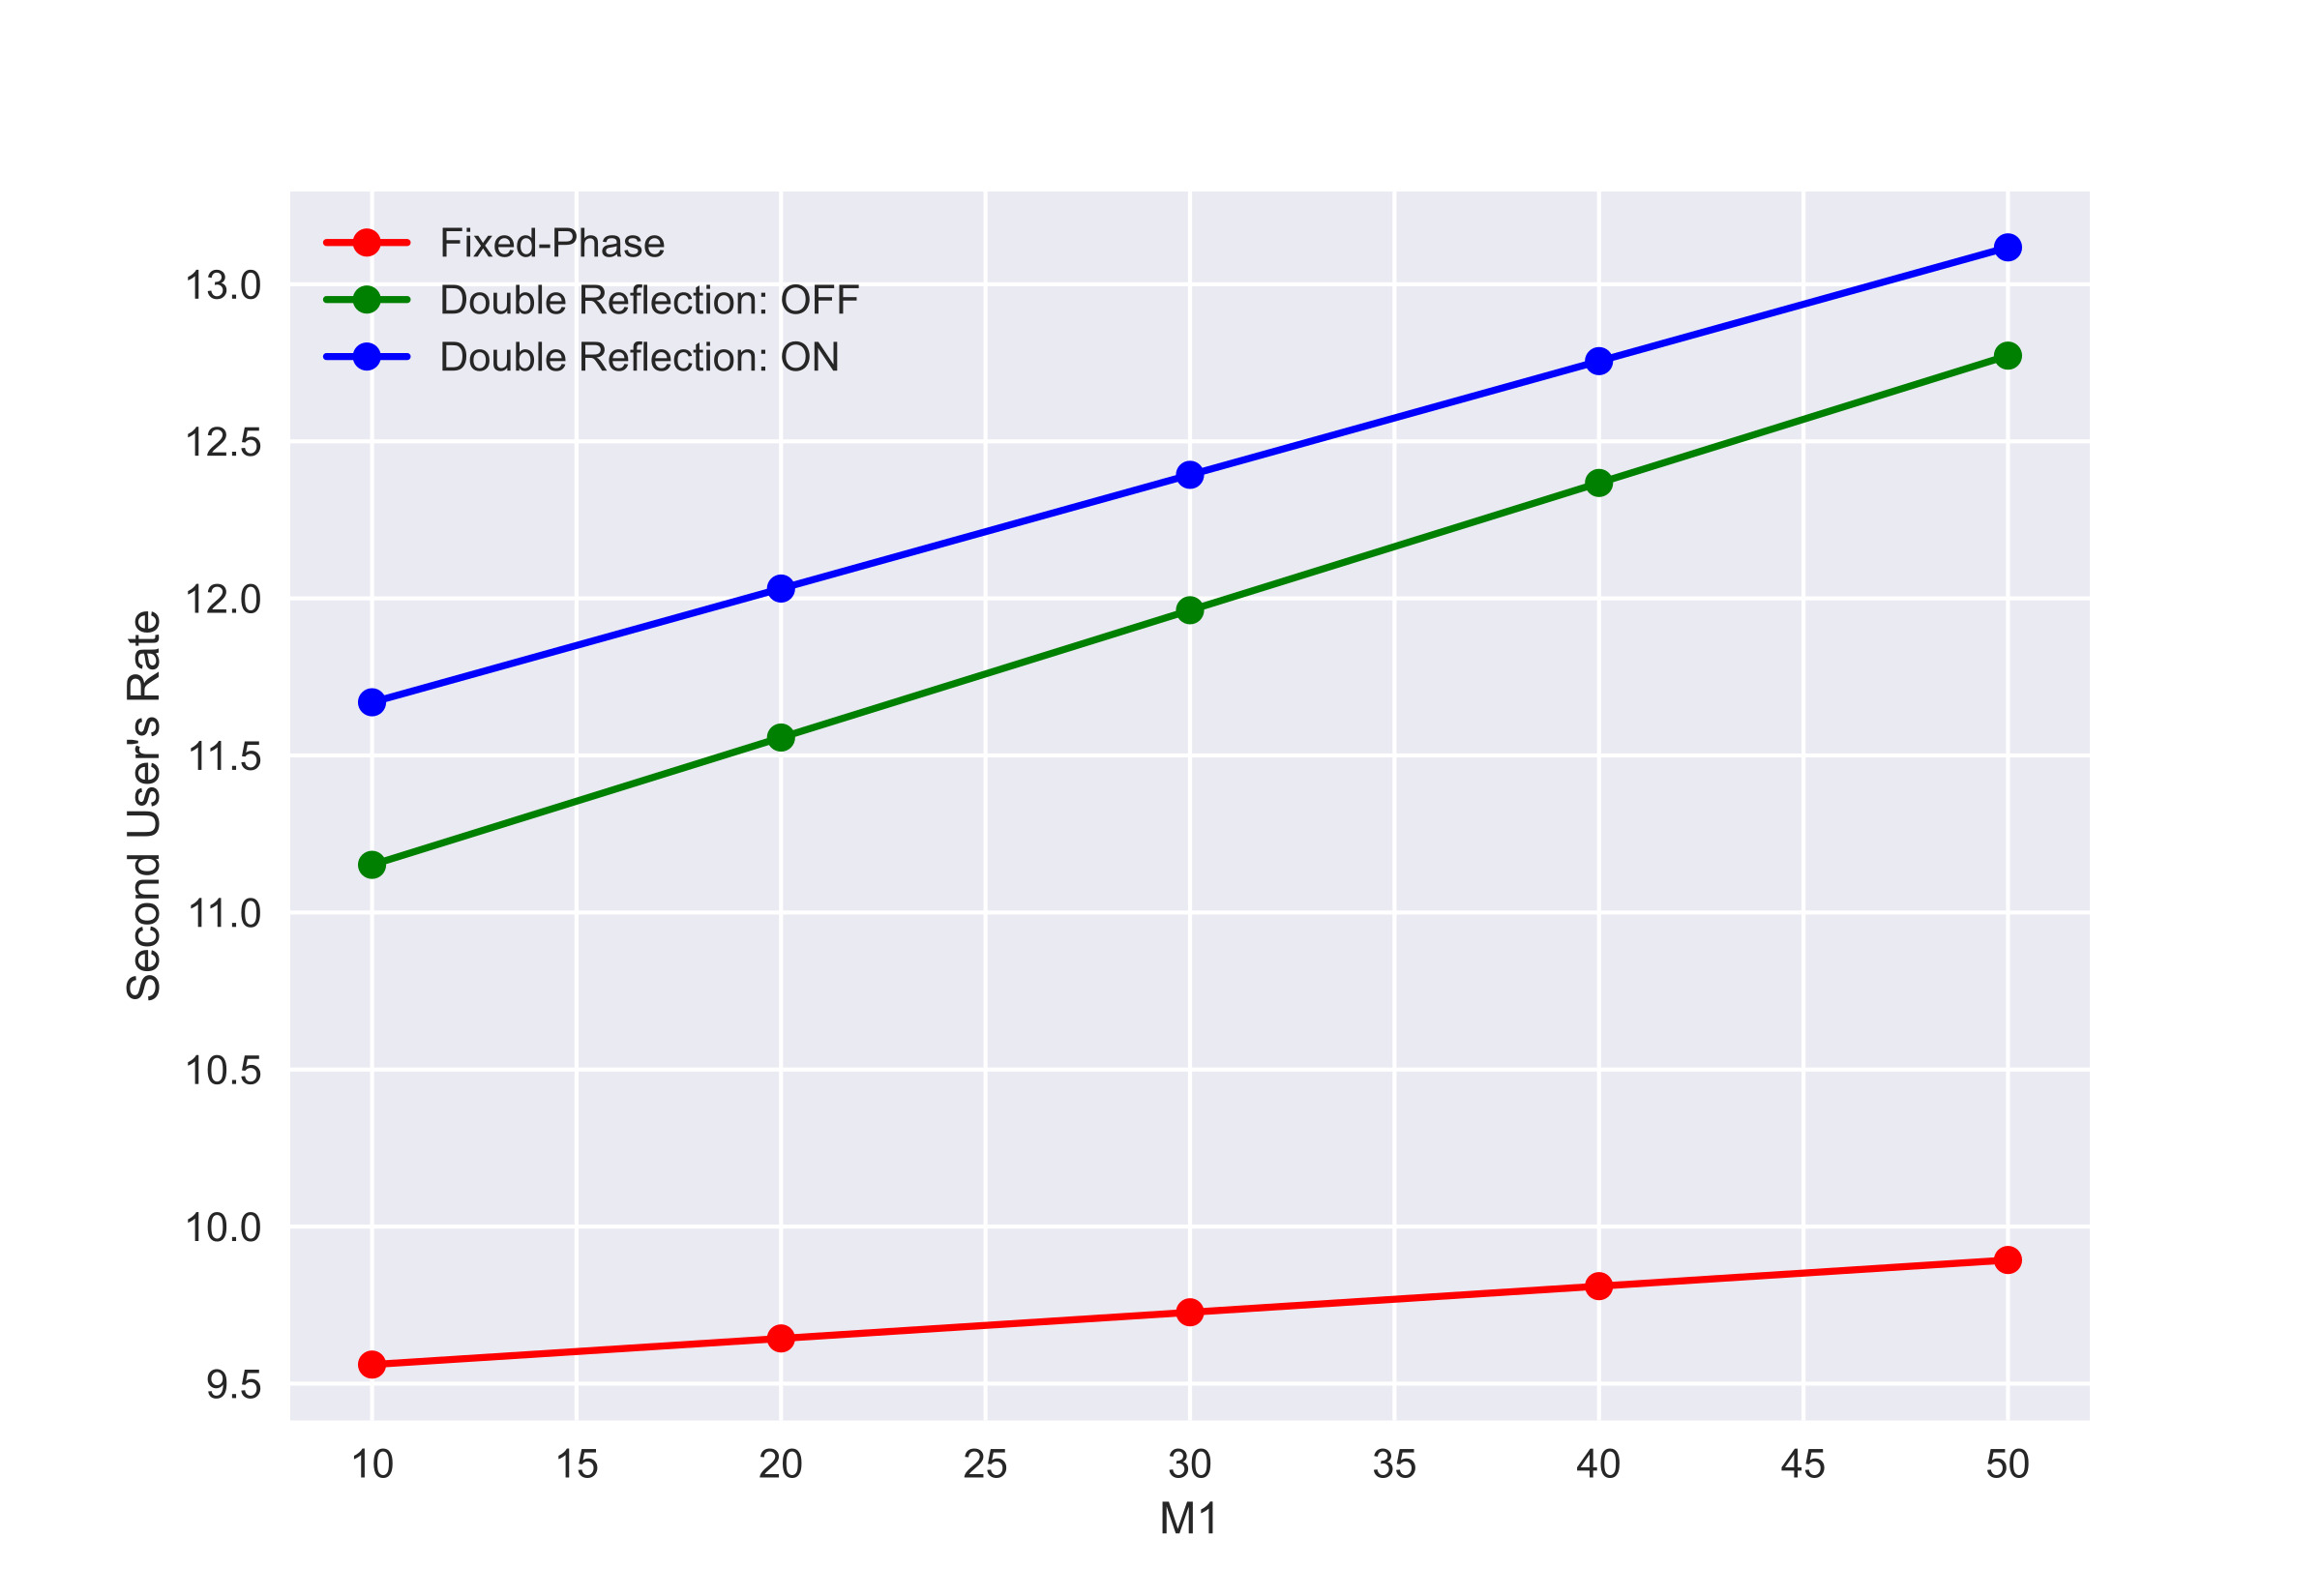
\includegraphics[width=0.95\linewidth]{No Blockage Second User's Rate}
		\caption{Second User's Rate}
	\end{minipage}
\end{figure}

\begin{figure}[!h]
	\centering
	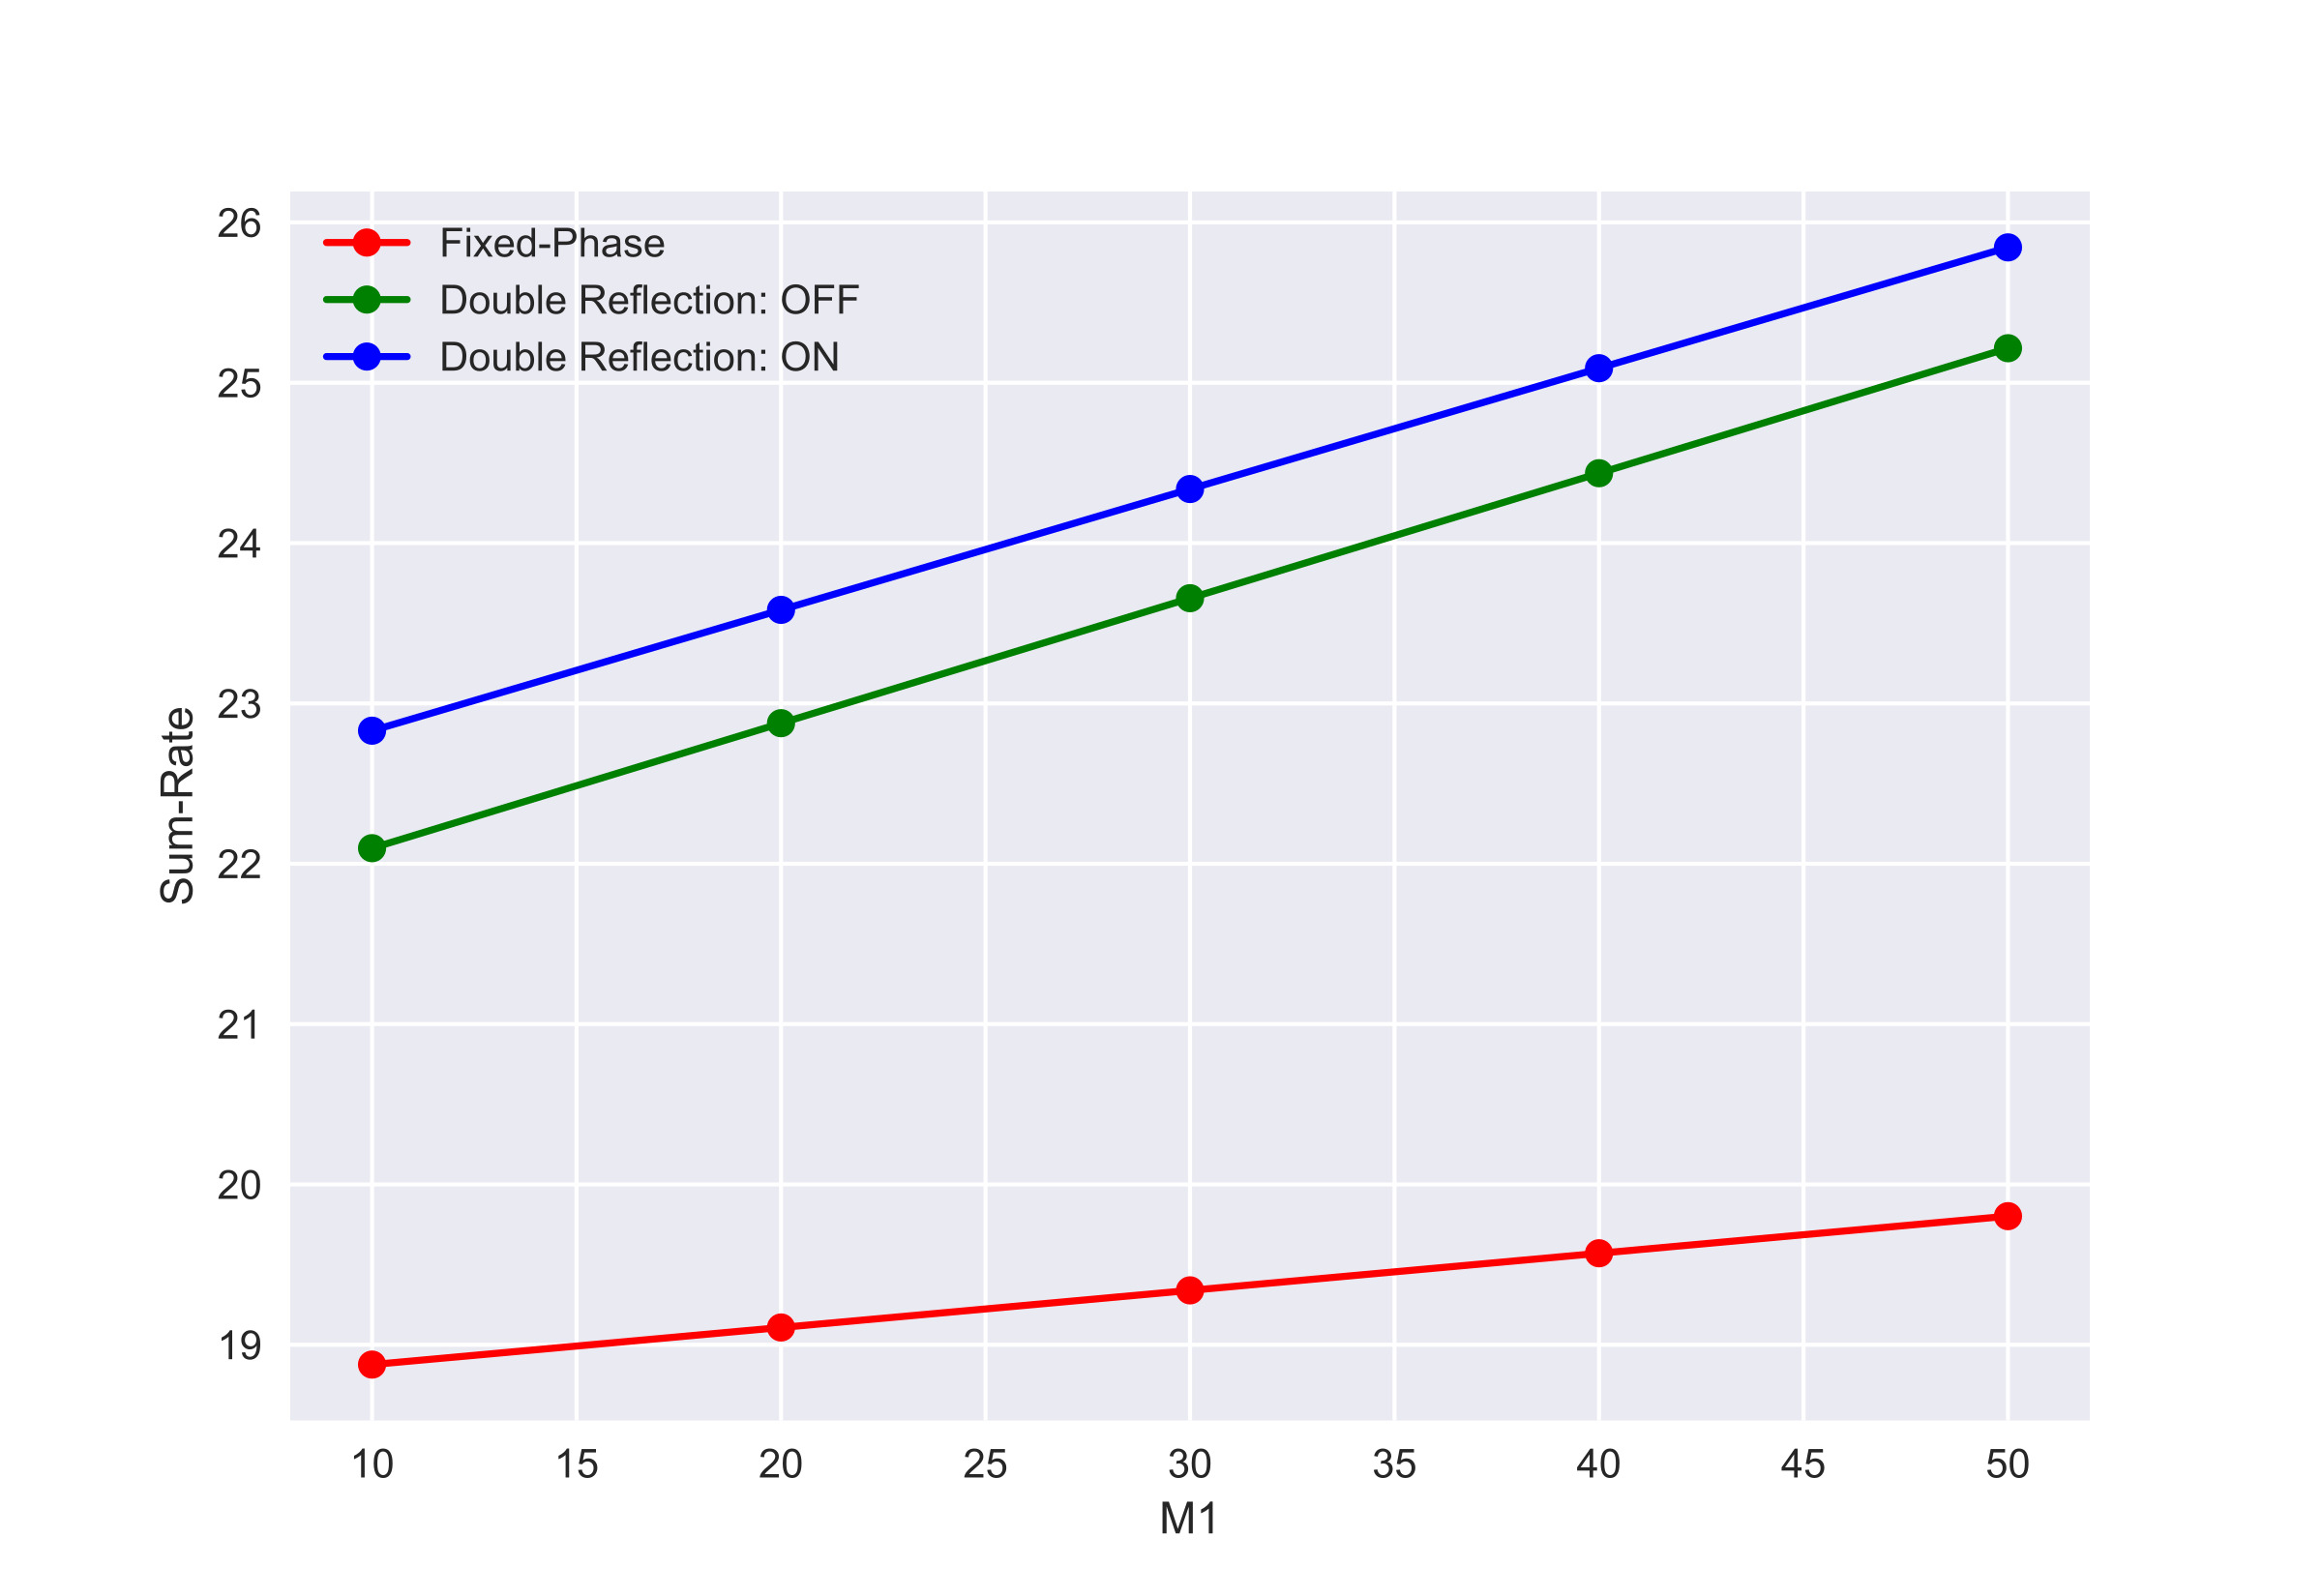
\includegraphics[width=0.95\linewidth]{No Blockage Sum-Rate}
	\caption{Sum-Rate}
\end{figure}

\subsubsection{Conclusion}
 As observed, in the scenario where the signal reflection between the surfaces is considered, both users experience an improvement in their received signals. However, it's essential to note that by considering signal reflection between the surfaces, we introduce complexity into the optimization process, leading to longer execution times. This complexity could potentially take the system out of real-time operation. Therefore, it is crucial for each individual to assess whether the improvement justifies the added complexity in their specific scenario.

\subsection{With Obstacle}
According to the conditions mentioned and in the presence of obstacles, simulations were conducted, and the following plots represent the user rates for User 1, User 2, and the total rate for both users:

\begin{figure}[!h]
	\centering
	\begin{minipage}{.5\textwidth}
		\flushleft
		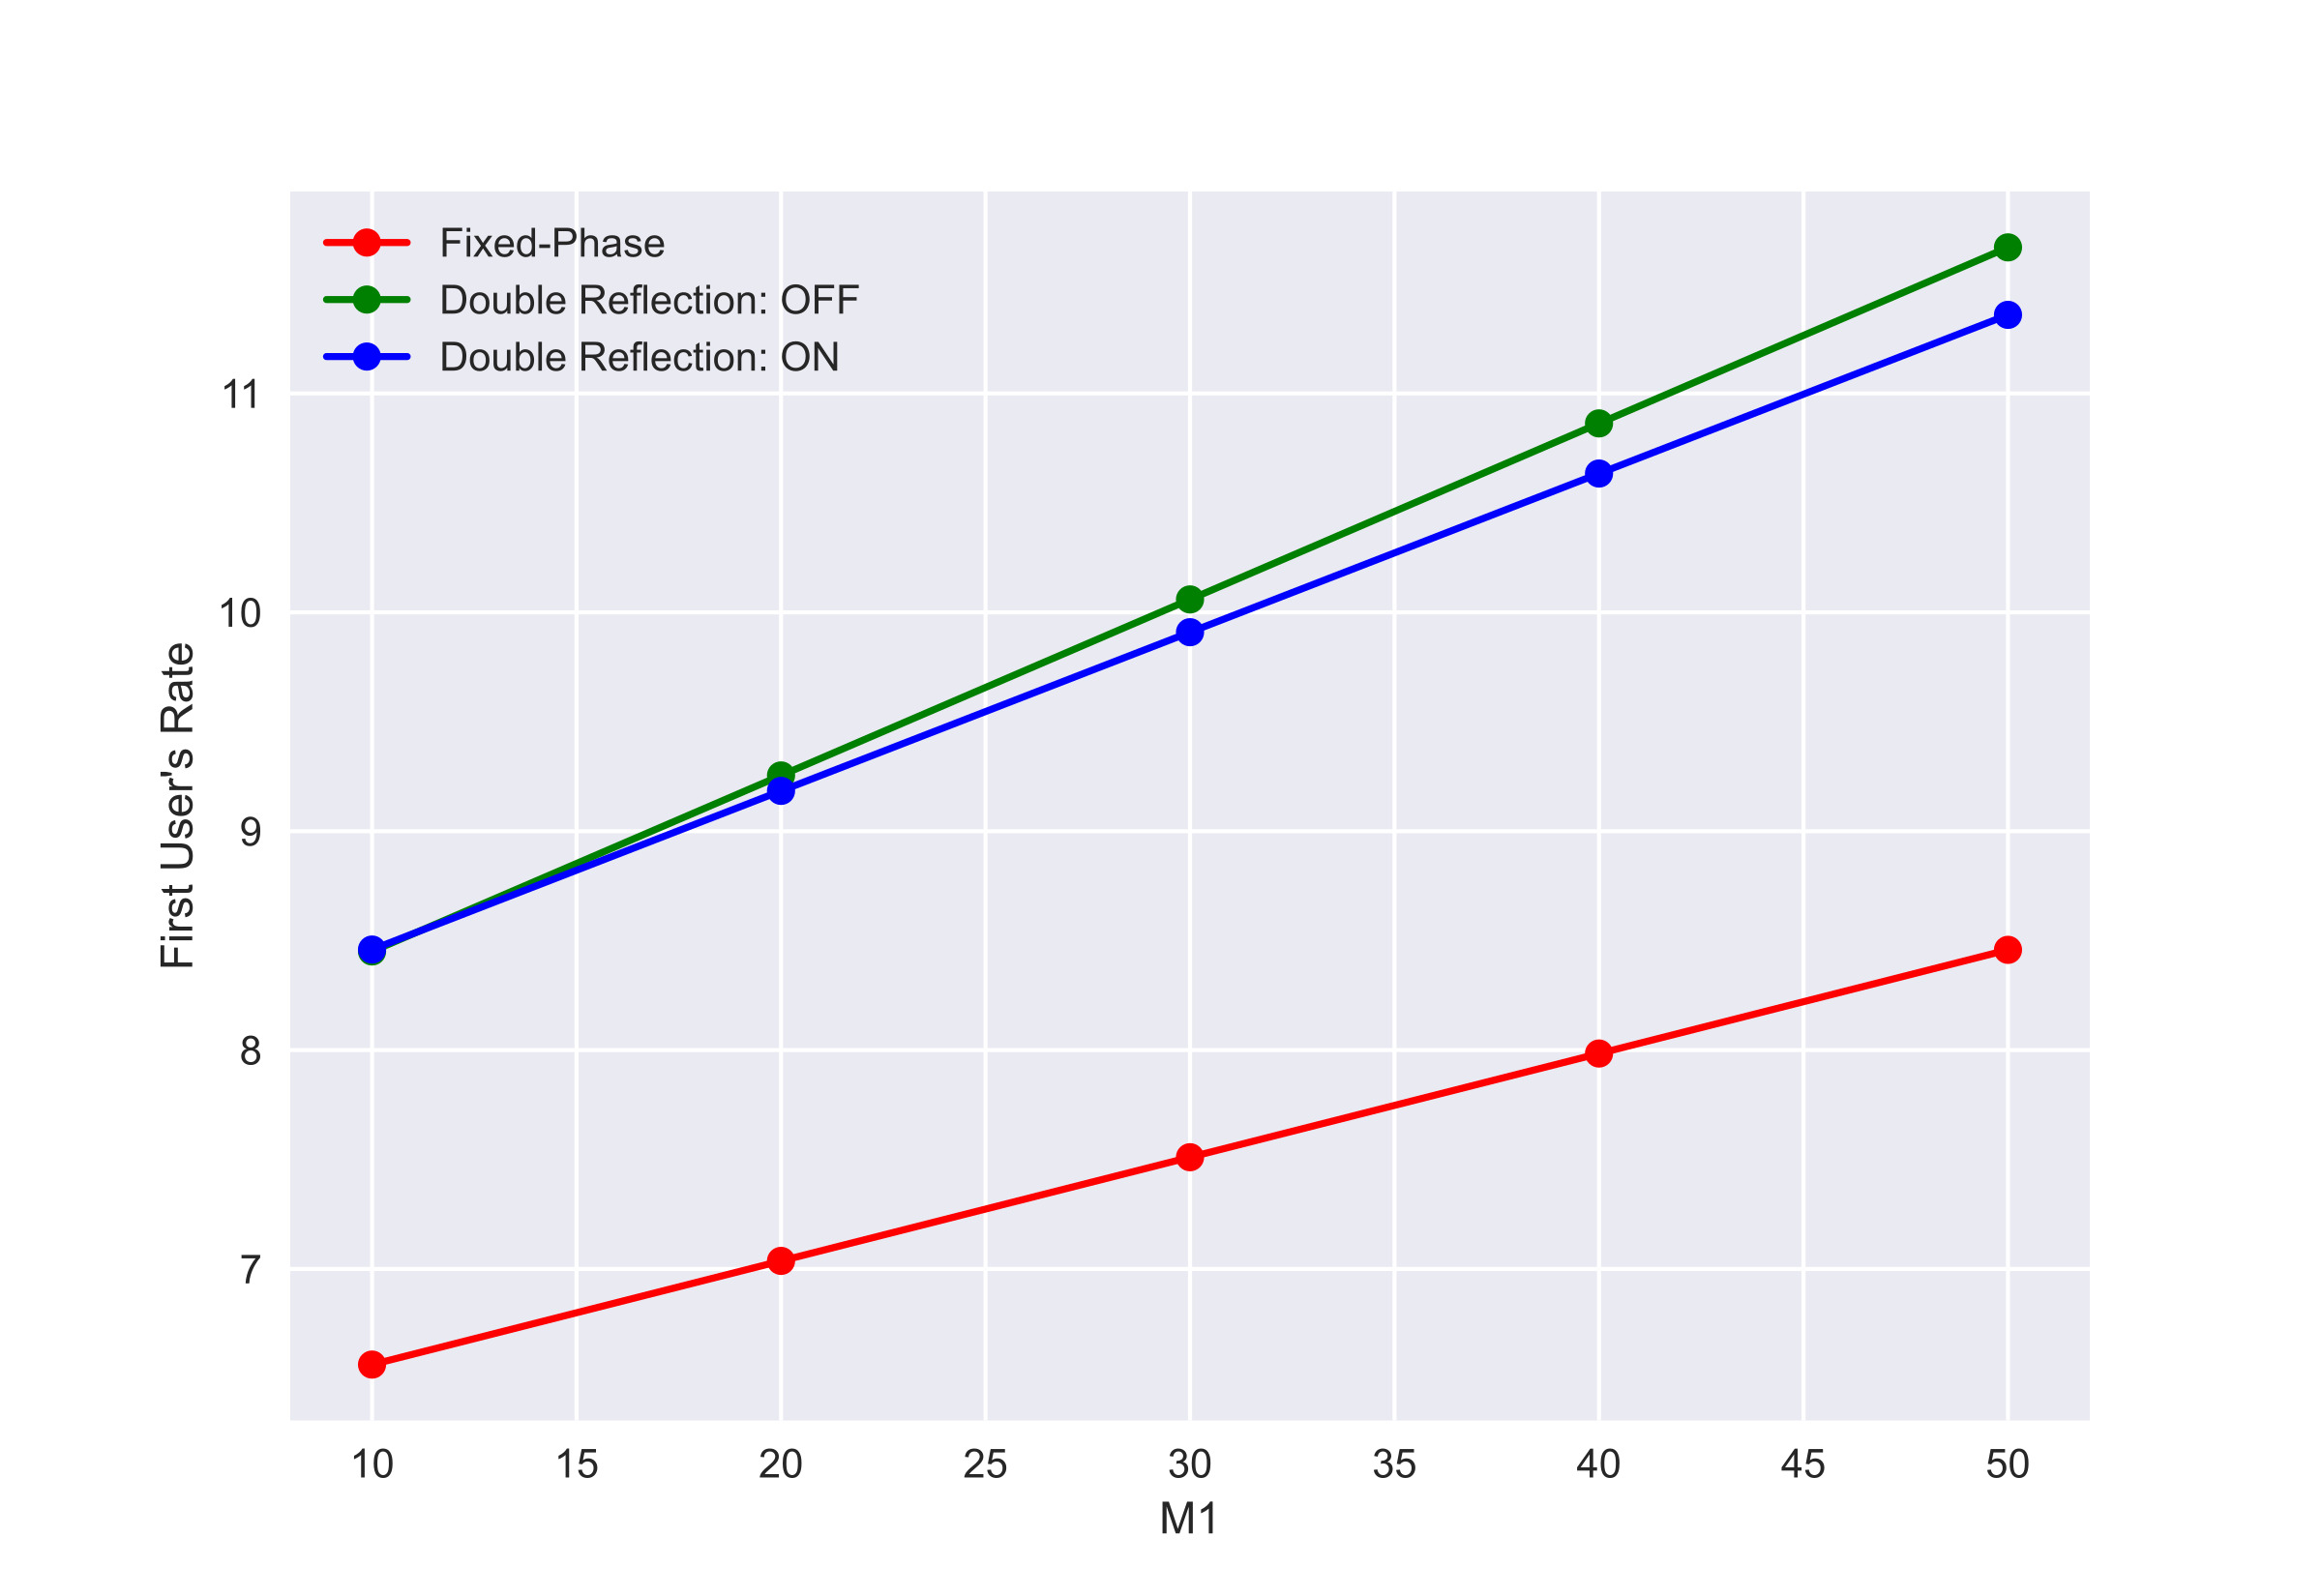
\includegraphics[width=0.95\linewidth]{With Blockage First User's Rate}
		\caption{First User's Rate}
	\end{minipage}%
	\vline
	\begin{minipage}{.5\textwidth}
		\flushright			
		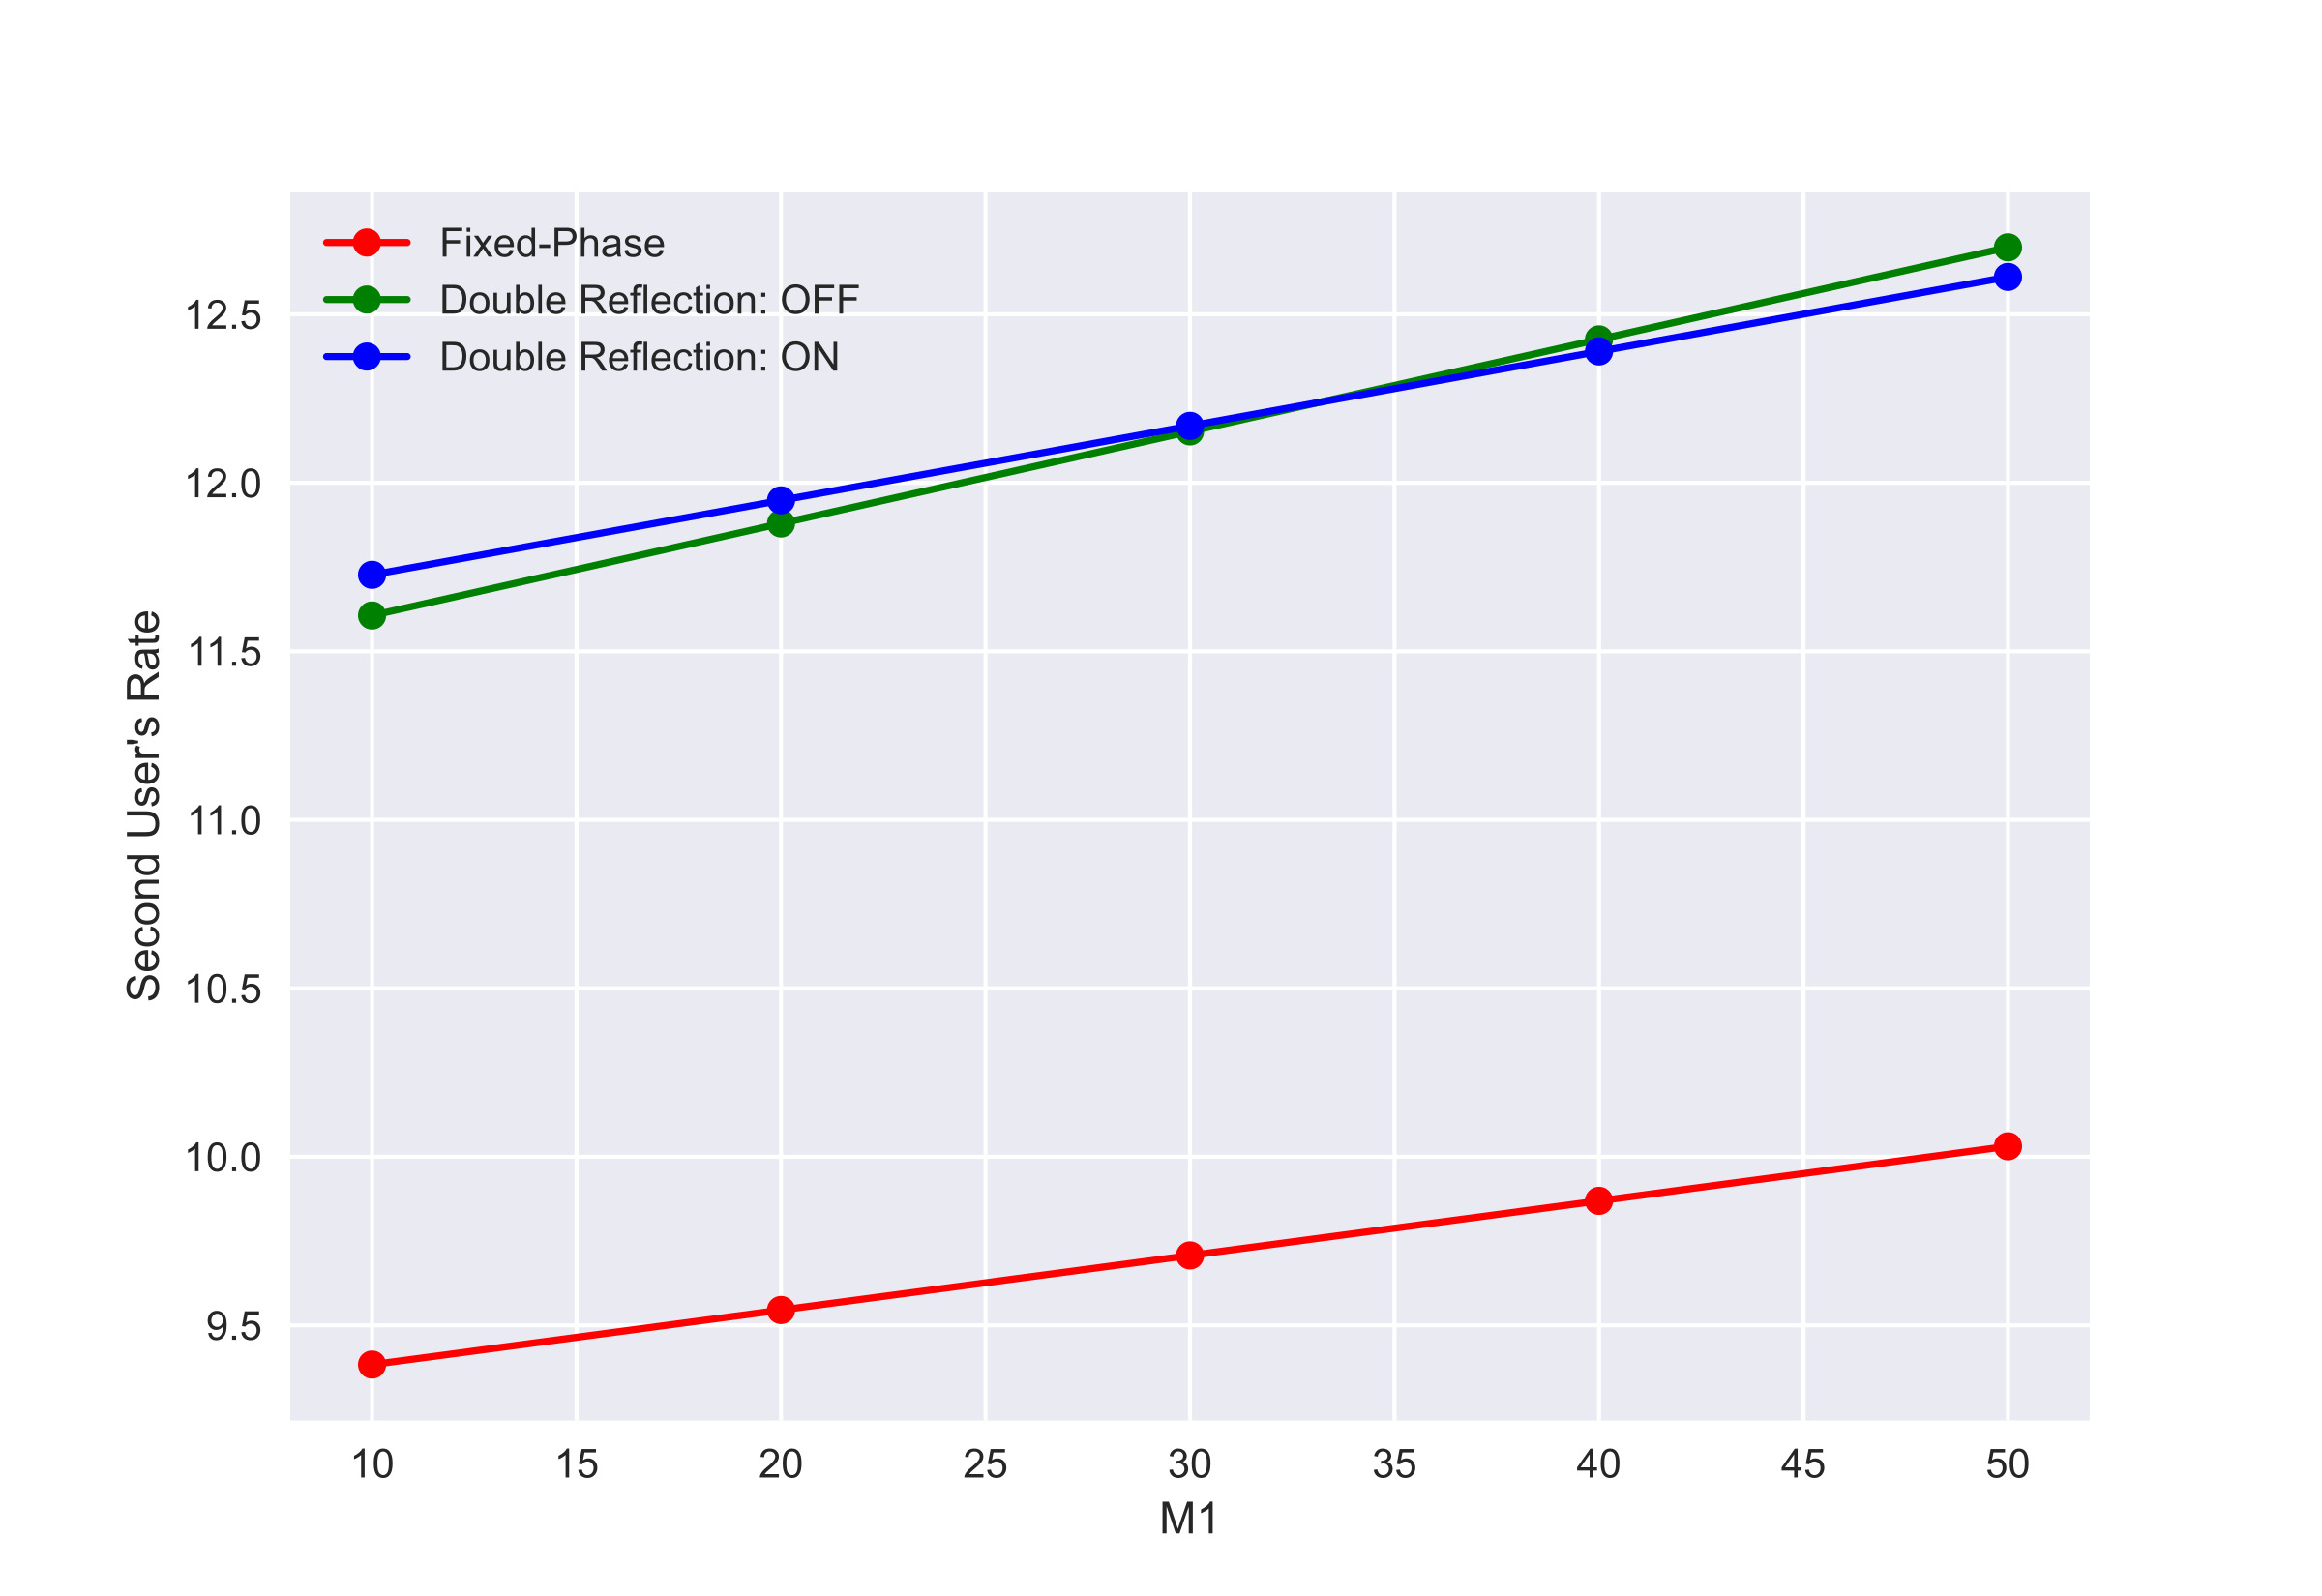
\includegraphics[width=0.95\linewidth]{With Blockage Second User's Rate}
		\caption{Second User's Rate}
	\end{minipage}
\end{figure}

\begin{figure}[!h]
	\centering
	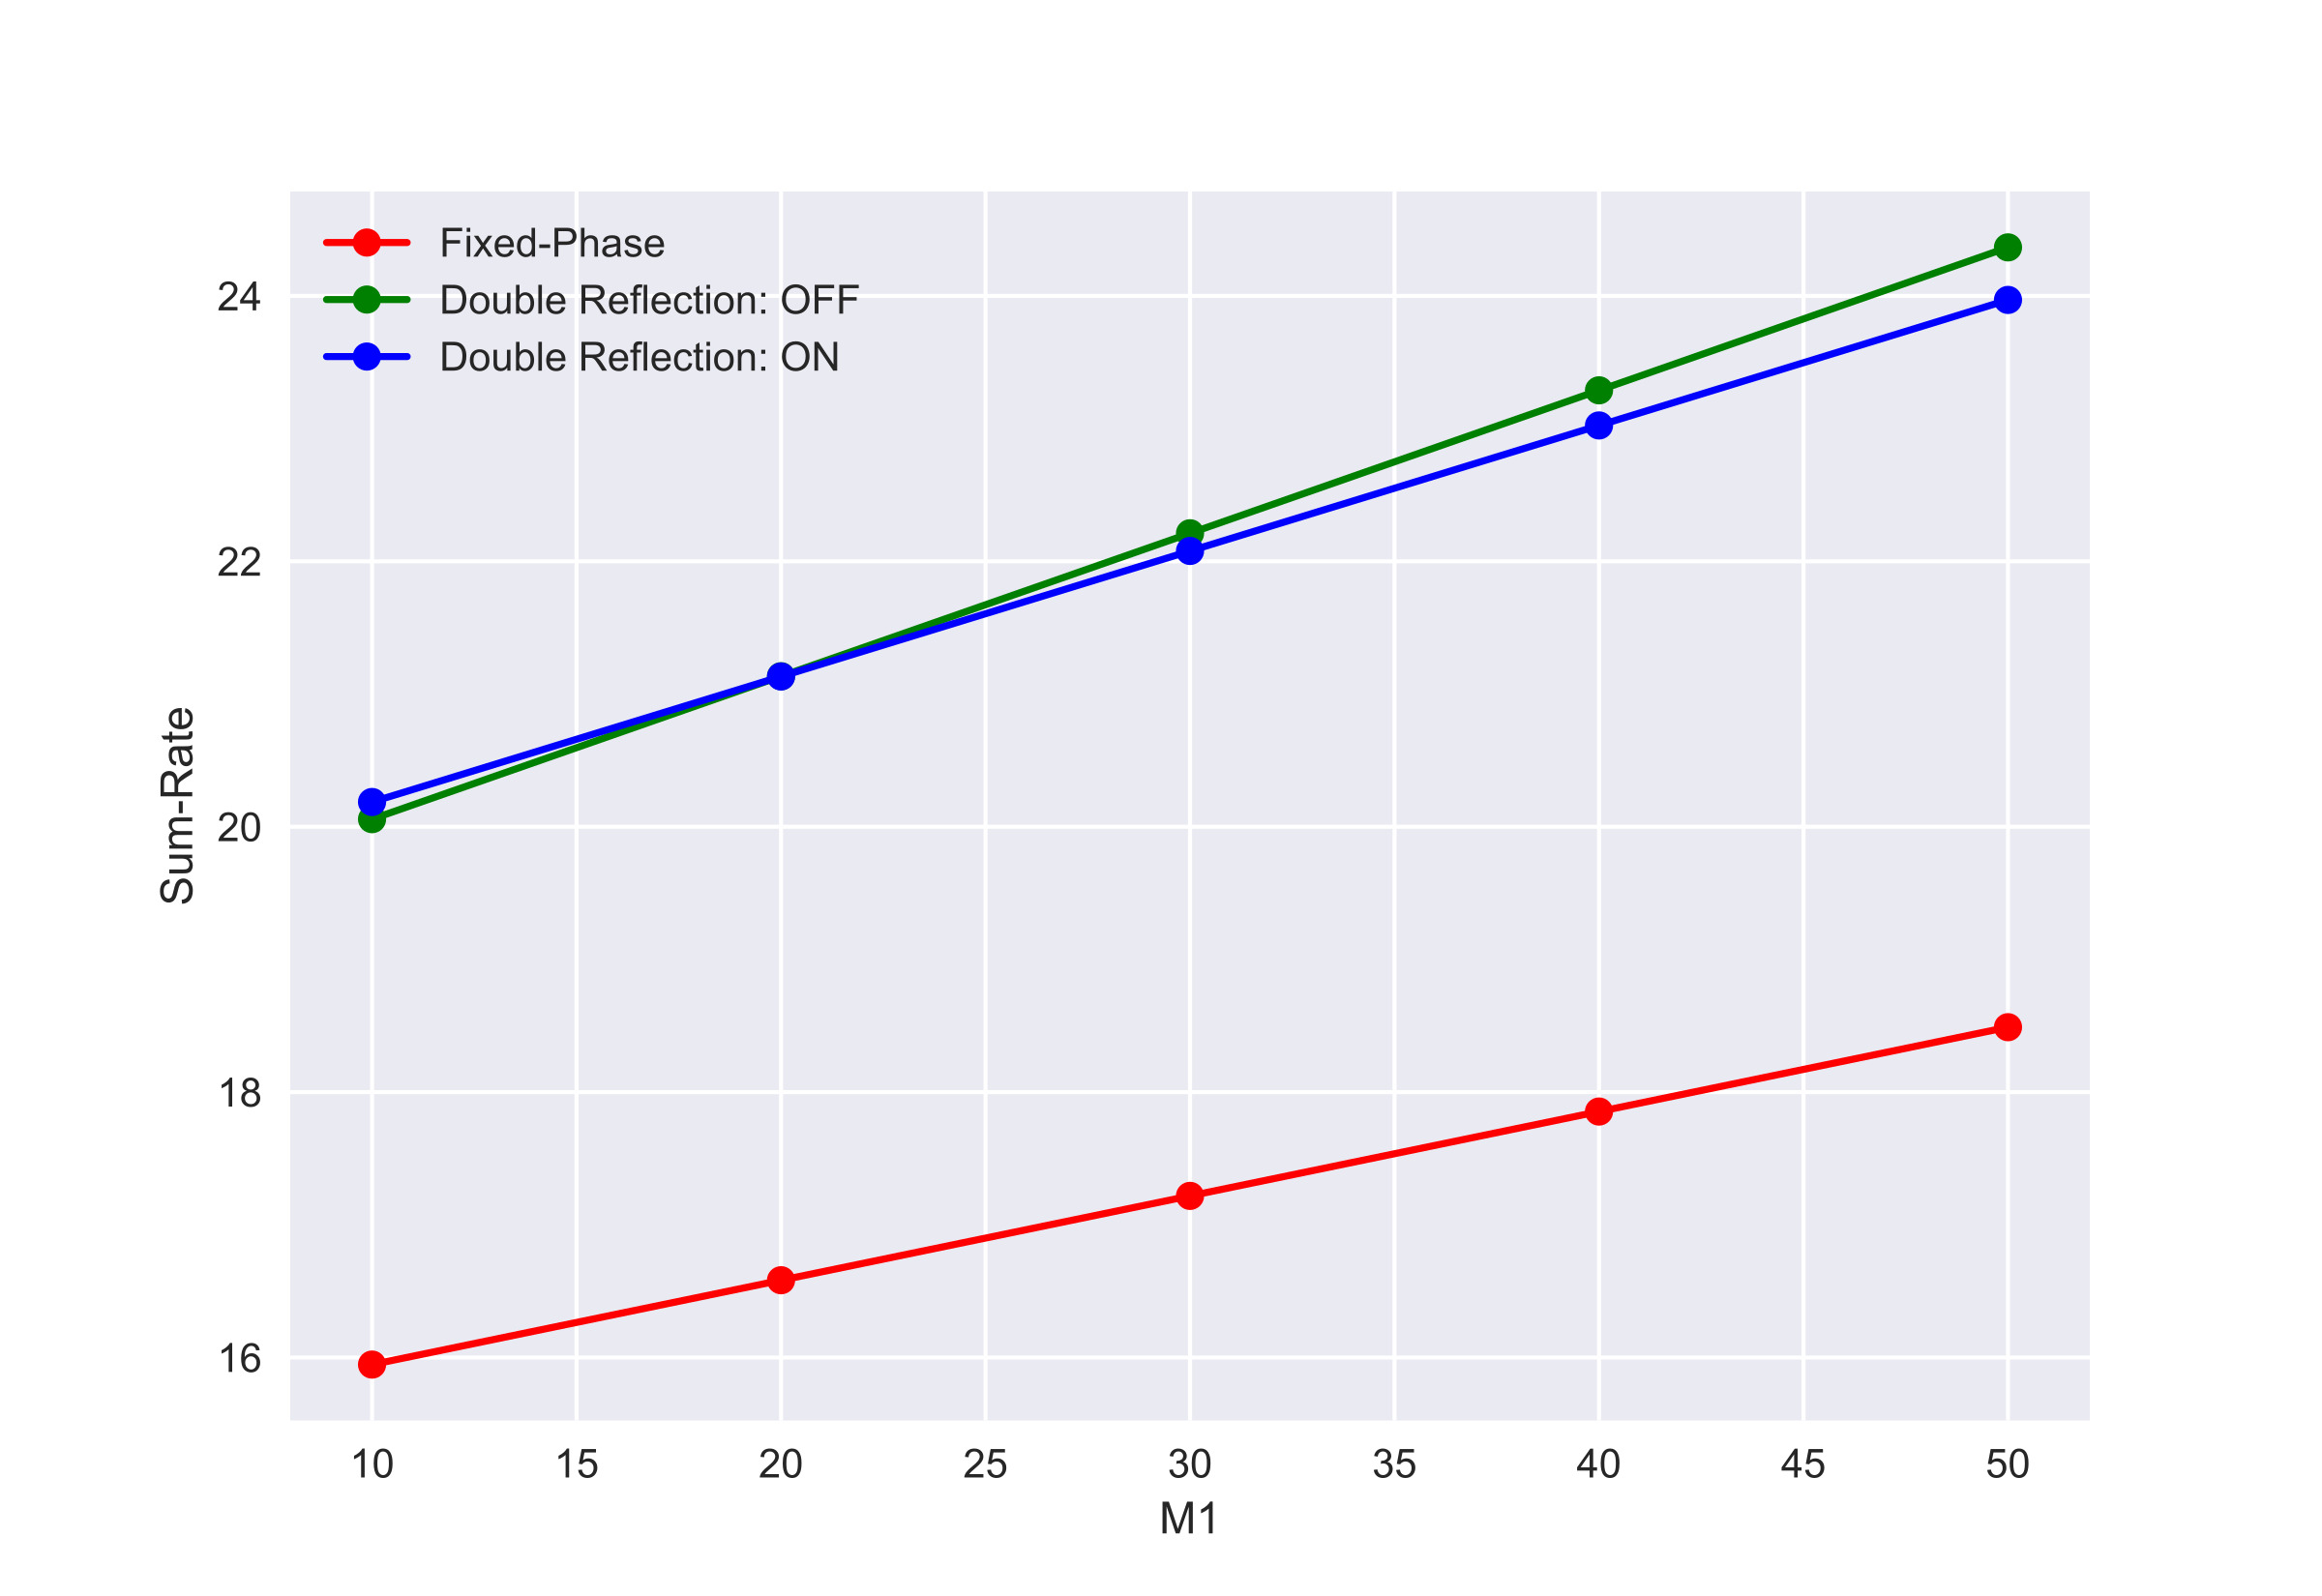
\includegraphics[width=0.95\linewidth]{With Blockage Sum-Rate}
	\caption{Sum-Rate}
\end{figure}

\subsubsection{Conclusion}
 As observed, in the scenario where signal reflection between surfaces is considered, neither of the users experiences any significant improvement in their received signals. Instead, it only adds complexity to the problem, leading to a reduction in the convergence rate of the optimization. Therefore, in this scenario and similar ones, the use of signal reflection between surfaces is not recommended, as it can increase computational load without providing any tangible improvements, ultimately reducing the convergence speed.

\section{Future Works}
In this section, we will explore three suggestions (future work) that could garner significant attention and potentially address various challenges:

\subsection{Second-order double reflection}
As discussed in this scenario, intelligent surface reflection has only been considered up to the first-order reflection. In the results section, it was observed that this reflection has a minimal impact on optimizing the output relative to the complexity it adds to the problem. However, there are situations where we are forced to consider this reflection. For example, when there is no direct line of sight to the transmitter and one of the two intelligent surfaces is not present, we are compelled to account for this reflection.

Now, one of the questions that arises is whether it is optimal in terms of user receiving rates to use second-order reflective signals when using three intelligent surfaces and not having a direct line of sight to two of them. This is one of the questions that can be answered in the future and can assist other researchers in their work.

\subsection{Creating a framework for optimizing IRS}
One of the main challenges in programming this project for optimizing phase coefficients was the absence of any specific framework for solving these problems. Initially, we had to search for an optimal algorithm and then implement that algorithm. There was a possibility that the chosen algorithm might get stuck in non-optimal local maxima and fail to reach an acceptable solution. It was even possible that the algorithm might not converge, in which case the researcher would be forced to explore other algorithms, which is not optimal in terms of time and energy.

Now, one of the future tasks could be designing a framework where users can input their scenarios, and this framework can test various conventional optimization methods in this field and select the optimal solution to present to us.

Of course, this task requires a significant amount of time and energy, and it is feasible primarily within the framework of an industrial project with appropriate funding.

\subsection{Finding the optimal step size}
One of the important issues in the convergence speed of the gradient descent algorithm is the choice of the step size. Research has been conducted for years on finding adaptive methods to determine the optimal step size. These algorithms can be implemented in this project to achieve better and faster results.

\bibliographystyle{unsrt}
\bibliography{references/references}  %%% Uncomment this line and comment out the ``thebibliography'' section below to use the external .bib file (using bibtex) .


%%% Uncomment this section and comment out the \bibliography{references} line above to use inline references.
% \begin{thebibliography}{1}

% 	\bibitem{kour2014real}
% 	George Kour and Raid Saabne.
% 	\newblock Real-time segmentation of on-line handwritten arabic script.
% 	\newblock In {\em Frontiers in Handwriting Recognition (ICFHR), 2014 14th
% 			International Conference on}, pages 417--422. IEEE, 2014.

% 	\bibitem{kour2014fast}
% 	George Kour and Raid Saabne.
% 	\newblock Fast classification of handwritten on-line arabic characters.
% 	\newblock In {\em Soft Computing and Pattern Recognition (SoCPaR), 2014 6th
% 			International Conference of}, pages 312--318. IEEE, 2014.

% 	\bibitem{keshet2016prediction}
% 	Keshet, Renato, Alina Maor, and George Kour.
% 	\newblock Prediction-Based, Prioritized Market-Share Insight Extraction.
% 	\newblock In {\em Advanced Data Mining and Applications (ADMA), 2016 12th International 
%                       Conference of}, pages 81--94,2016.

% \end{thebibliography}


\end{document}
